\begin{itemize}
	\item The dataset collects multiple features related to each passenger-flight, including labels for whether the passenger was satisfied with the flight or not.
	\item It has 24 columns (22 + id + result).
	\item Id column is dropped (it would add weight).
	% TODO: add reference to missing values treatment
	\item Observation: the only column with null values is 'arrival\_delay\_in\_minutes', with 393 missing values.
	\item Categorical columns: 4
	\subitem \underline{Features and possible values}: Gender (2), customer\_type (2), type\_of\_travel (2), customer\_class (3)
	\subitem \underline{Decision}: use one-hot encoding in all of them (none of them is a clear candidate for being weighted)
	\item Looking for strong correlations: pairwise correlation function to check if two features show strong correlation.
	\subitem NOTE: 'satisfaction' (the label we will try to predict) is not strongly correlated ($>$0.7) with any of the other features. 
	\subitem \emph{arrival\_delay\_in\_minutes} and \emph{departure\_delay\_in\_minutes} have the highest correlation rate (0.965291), which semantically makes sense; all other variables are less than 75\% correlated.
	\subitem \begin{center}
		\captionsetup{type=figure}
		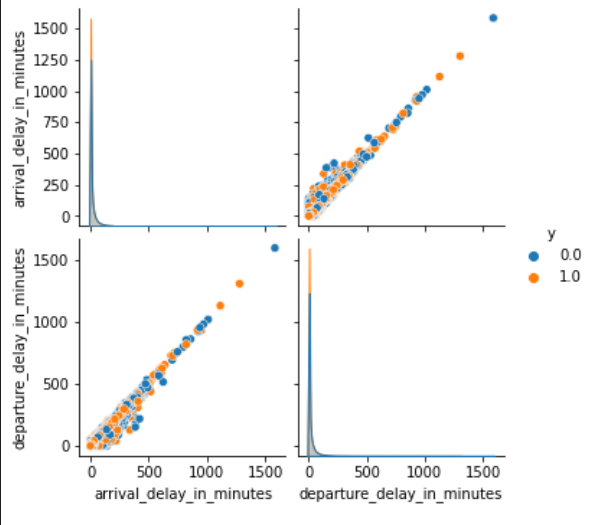
\includegraphics[width=250px]{correlation.png}
		\captionof{figure}{Correlation between most-correlated features}
	\end{center}
\end{itemize}